\section{Auswertung}

Alle Ausgleichsrechnungen werden mit dem Paket \texttt{scipy.optimize.curve\_fit}  aus \texttt{Python 3.7.3} durchgeführt.
Für Rechnungen mit fehlerbehafteten Größen wird das Paket \texttt{uncertainties} aus \texttt{Python 3.7.3} verwendet.\\

\subsection{Justage}
Zunächst wird eine Temperaturmessung und Justage durchgeführt. Mithilfe eines digitalen Thermometers wird die Temperatur 
auf \SI{21.5}{\degreeCelsius} bestimmt. Nach dem Einstellen der in der Versuchsanleitung \cite{anleitung} aufgeführten Startwerte
werden diese solange variiert bis die gewünschten Signale zu sehen sind.
Die richtige Frequenz ist daran zu erkennen, dass das gemessene Signal keine Schwingungen mehr aufweist. Ist die richtige Frequenz
eingestellt und es wird die Phase variiert ist es das Ziel, dass sich das gesamte Signal ausschließlich im Realteil befindet.
Das bedeutet es wird versucht die Phase so verändern, dass eines der beiden angezeigten Signale möglichst verschwindet.
Beim Eintsellen der Gradienten ist darauf zu achten, dass das Signal möglichst lange zu erkennen ist. 
Unter Berücksichtigung dieser Vorgehensweisen ergeben sich
\begin{align}
  \text{Frequenz}&=\SI{221.72088}{\mega\hertz} \\
  \text{Phase} &= \SI{30}{\degree} \\
    x&=–1.7 \\
    y&=–5.1 \\
    z&=3.7 \\
    z^2 &=–2.4
\end{align} \noindent
für die einzustellenden Werte. \\
Die Bestimmung der Pulslängen für den $\SI{90}{\degree}$- und $\SI{180}{\degree}$-Puls ergeben
\begin{align}
  \SI{180}{\degree} &= \SI{5.04}{\micro\second}\\
  \SI{90}{\degree}  &= \SI{2.52}{\micro\second}
\end{align} \noindent

\subsection{$T_1$-Messung}
Zur Bestimmung der $T_1$-Zeit wird die Magnetisierung für verschiedene Pulsabstände $\tau$ bestimmt. 
Eine solche Messung ist beispielhaft in Abbildung \ref{fig:t1} dargestellt. Deutlich wird, dass eine vollständige Unterdrückung
der Imaginärteils, dargstellt durch den grünen Graphen, nicht gelungen ist. Außerdem sind zwei Ausschläge zu erkennen, wobei der 
erste dem $\SI{180}{\degree}$-Puls zuzuordnen ist und der zweite dem $\SI{90}{\degree}$-Puls, der in diesem 
Versuchsteil untersucht werden soll.
\begin{figure}[H]
  \centering
  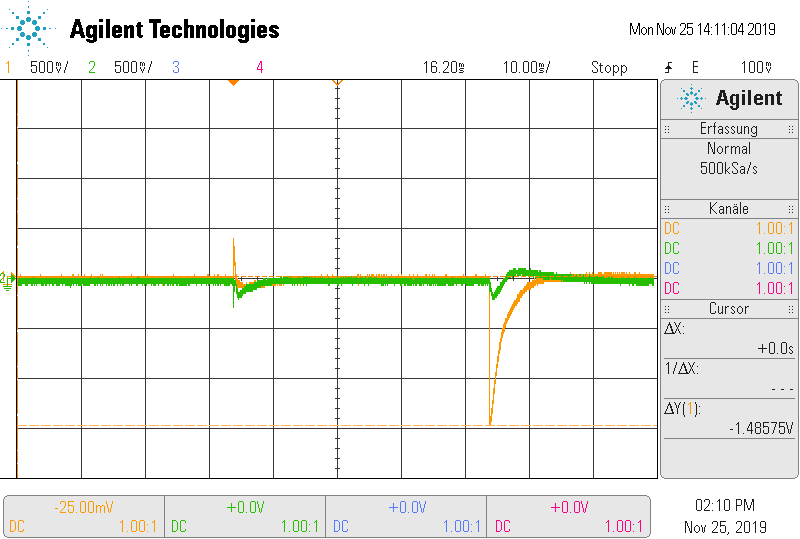
\includegraphics[width=0.8\textwidth]{../data/T1.png}
  \caption{Beispielhafte Darstellung einer Messung zur Bestimmung der T1-Relaxationszeit. Untersucht wird der zweite zu 
  erkennende Ausschlag, da er dem $\SI{90}{\degree}$-Puls zugeordnet ist. Beachtet wird dabei nur der Realteil des Signals, 
  der durch den orangenen Graphen repräsentiert wird.}
  \label{fig:t1}
\end{figure} \noindent
Die bei der Messung mithilfe der Cursorfunktion bestimmten Signalstärken sind in Abbildung \ref{fig:t1_fit} gegen den
jeweiligen Pulsabstand $\tau$ aufgetragen. 
\begin{figure}[H]
  \centering
  \includegraphics[width=0.9\textwidth]{../Auswertung/t1_fit.pdf}
  \caption{Die aufgenommen Messwerte der Signalstärke in Abhängigkeit der Pulslänge $\tau$, sowie die 
  zur Bestimmung der $T_1$-Zeit durchgeführte Ausgleichskurve.}
  \label{fig:t1_fit}
\end{figure}
Durch die aufgenommenen Messwerte wird ein Ausgleichgraph der Form
\begin{equation}
  M(\tau) = M_0 \cdot \exp(–\tau/T_1) + M_1
\end{equation}
gelegt. Diese Regression liefert 
\begin{align}
  T_1 &= \SI{1.35(005)}{\second} \\
  M_0 &= \SI{3.00(005)}{\volt} \\
  M_1 &= \SI{-1.40(005)}{\volt}
\end{align} \noindent
für die Relaxationszeit $T_1$, sowie die Magnetisierungsparameter $M_0$ und $M_1$.
Idealerweise stehen die Parameter $M_0$ und $M_1$ im Zusammenhang von $M_0 = -2M_1$. Bei den durch die Regession bestimmten
Werten ergibt sich ein Verhätnis von
\begin{equation}
  \frac{M_0}{M_1} = 2.22.
\end{equation}
Das bedeutet, dass durch die durchgeführte Justage nicht die exakten Einstellungen vorgenommen worden sind. Dies lässt
sich zum Einen auch schon daran erkennen, dass sowohl Real- als auch Imaginärteil noch zu erkennen sind, der Wert liegt jedoch
noch im Rahmen.

\subsection{$T_2$-Messung}
Im ersten Versuchsteil zur Bestimmung der $T_2$-Zeit wird der \textit{MG}-Schalter auf \textit{on} gestellt. Somit 
wird hier die Meiboom-Gill-Methode angewendet.
In Abbildung \ref(fig:t2) ist das aufgenommene Signal dargestellt. Es ist gut zu erkennen, dass das Signal bei 
dem eingestellten Pulsabstand von $\tau=\SI{1}{\second}$ HIER FEHLT DER ECHTE WERT den gewünschten Verlauf zeigt.
\begin{figure}[H]
  \centering
  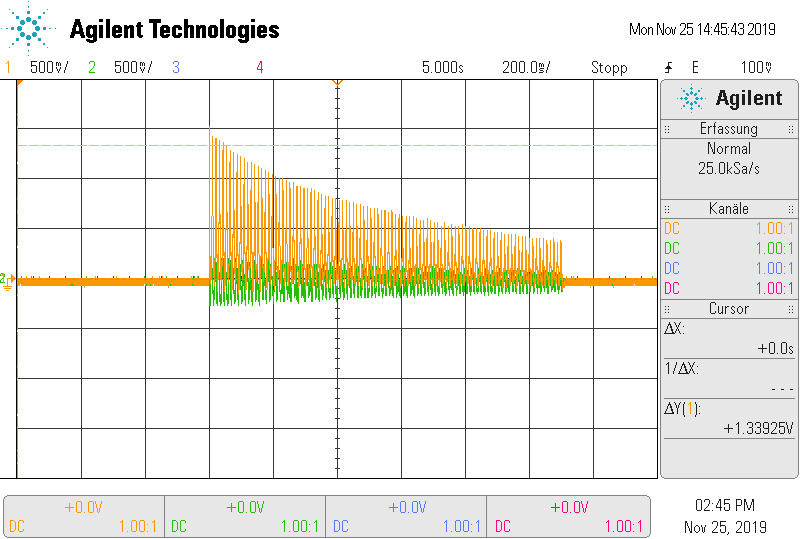
\includegraphics[width=0.8\textwidth]{../data/T2.png}
  \caption{Das aufgenommene Signal zeigt bei der Meiboom-Gill-Methode mit $\tau=\SI{1}{\second}$ HIER FEHLT MIR EIN WERT den gewünschten Verlauf. Die Signalstärke ist nach dem
  100.Maximum auf ca. $\frac{1}{3}$ der Maximalhöhe abgefallen.}
  \label{fig:t2}
\end{figure} \noindent
Zur Bestimmung der Relaxationszeit $T_2$, wird eine Ausgleichskurve der Form
\begin{equation}
  M(t) = M_0 \cdot \exp(–t/T_2) + M_1
\end{equation}
an die Einhüllende des oszilliereden Signals angepasst. Diese ist zusammen mit den Messwerten in Abbildung \ref{fig:T2_fit}
dargestellt.
\begin{figure}[H]
  \centering
  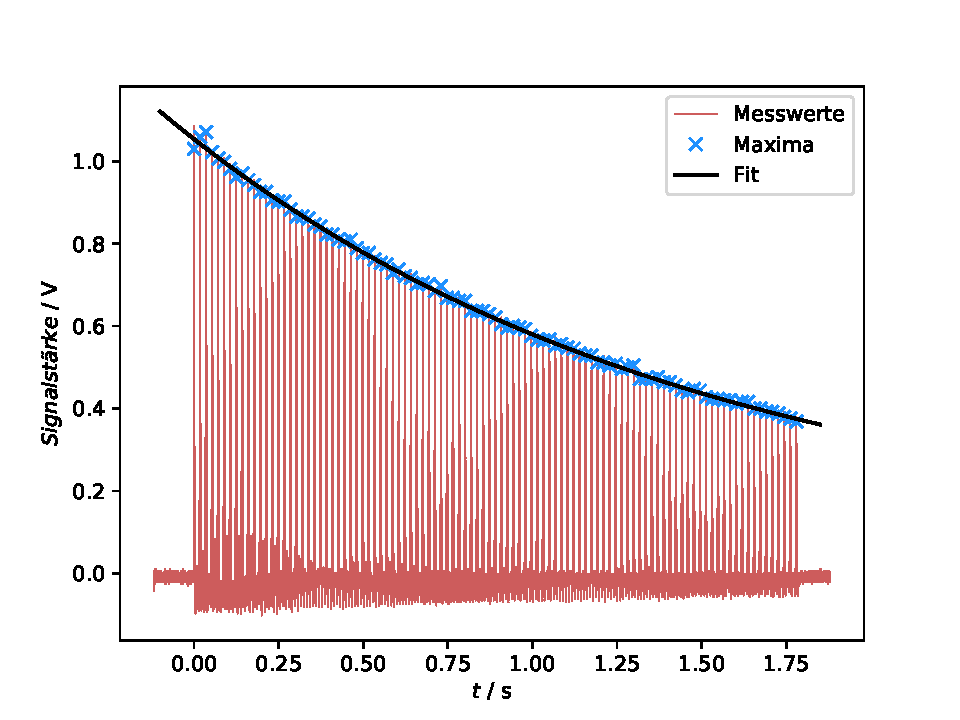
\includegraphics[width=0.9\textwidth]{../Auswertung/T2_fit.pdf}
  \caption{Die zur Bestimmung der $T_2$-Zeit durchgeführte Ausgleichsrechnung. In Blau ist die Ausgleichskurve zu erkennen,
  die an die Einhüllende des oszillierenden Signals angepasst wird.}
  \label{fig:T2_fit}
\end{figure} \noindent
Die Regression liefert
\begin{align}
  M_0 &=  \SI{0.99(001)}{\volt} \\
  M_1 &=  \SI{0.067(002)}{\volt} \\
  T_2 &=  \SI{1.53(004)}{\volt}
\end{align}
für die gesuchten Parameter. \\
Im Vergleich dazu ist in Abbidung \ref{fig:t2_off} das aufgenommene Signal für die Carr-Purcell-Methode zu sehen. Das heißt bei der 
Messung ist der \textit{MG}-Schalter auf \textit{off} gestellt.
\begin{figure}[H]
  \centering
  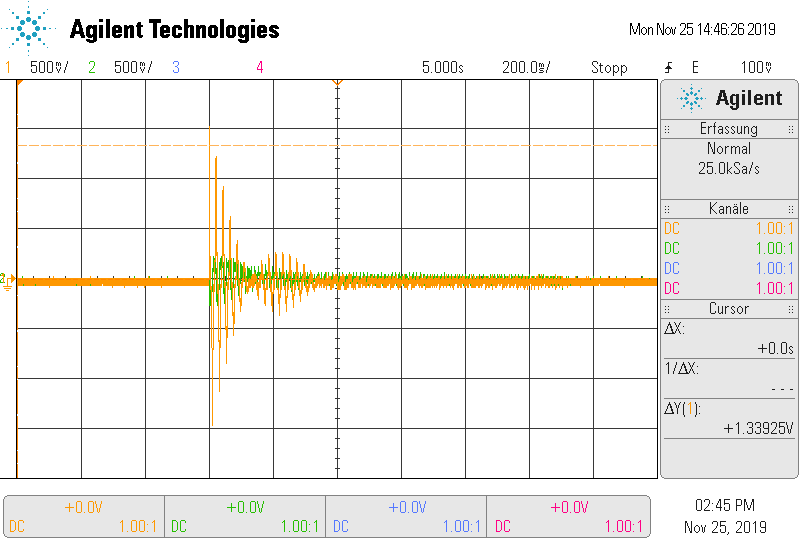
\includegraphics[width=0.8\textwidth]{../data/scope_76.png}
  \caption{Das aufgenommene Signal für die Carr-Purcell-Methode. Dabei ist deutlich zu erkennen, dass es durch die 
  $\SI{180}{\degree}$-Pulsen zum Wechsel zwischen Maxima im positiven und negativen Bereich kommt.}
  \label{fig:t2_off}
\end{figure} \noindent
Es wird deutlich, dass im Gegensatz zu dem aufgenommenen Signal der Meiboom-Gill-Methode bei dieser Aufnahme die Maxima zwischen
dem positiven und negativen Bereich alternieren. Dies ist auf die geschalteten $\SI{180}{\degree}$-Pulse zurückzuführen. Jedoch
nimmt auch bei dieser Messmethode die Signalstärke mit der Zeit ab. \\
Zur Verdeutlichung des typischen Verlaufs eines solchen Signals is in Abbildung \ref{fig:N1} ein Signal dargestellt mit nur einem
geschalteten B-Puls.
\begin{figure}[H]
  \centering
  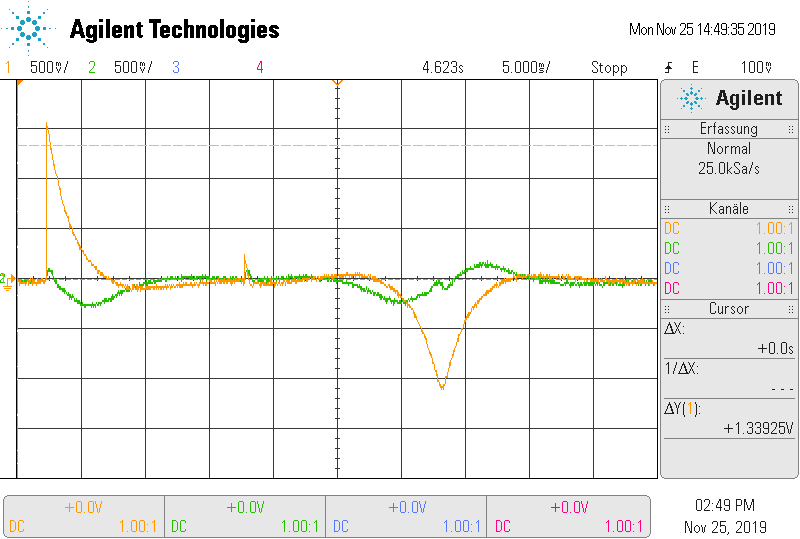
\includegraphics[width=0.8\textwidth]{../data/scope_77.png}
  \caption{Das aufgenommene Signal, wenn nur ein einziger B-Puls geschaltet ist. Zu Beginn des Signals ist der 
  $\SI{90}{\degree}$-Puls zu erkennen. Nach dem $\SI{180}{\degree}$-Puls baut sich das Signal durch die Rephasierung 
  wieder auf.}
  \label{fig:N1}
\end{figure} \noindent
Zu erkennen ist zu Beginn des aufgenommenen Signals der $\SI{90}{\degree}$-Puls, der die Magnetisierung in die x-y-Ebene kippt.
Daraufhin kommt es zur Dephasierung der Spins mit der $T_2$-Zeit. Der $\SI{180}{\degree}$-Puls, der durch einen kleinen Ausschlag
zwischen dem Maximum und Minimum zu erkennen ist, sorgt für eine Rephasierung. Diese führt zu einem messbaren Signal, welches 
jedoch aufgrund der Spin-Gitter-Wechselwirkung eine geringe Signalstärke aufweist.

\subsection{Diffusionsmessung}
In Abbildung \ref{fig:diff_fit} sind die gemessenen Echohöhen gegen den Pulsabstand $\tau$ auftragen.
Zusätzlich dazu wird eine Ausgleichskurve der Form
\begin{equation}
  M(\tau) = M_0 \cdot \exp(–2\tau/T_2)\cdot \exp(–\tau^3/T_D) + M_1 
\end{equation}
mithilfe der Messwerte bestimmt. Dabei beschreibt $T_D$ die Diffusionszeit. Zur Bestimmung der gesuchten Parameter wird 
die zuvor bestimmte $T_2$-Zeit verwendet.
\begin{figure}[H]
  \centering
  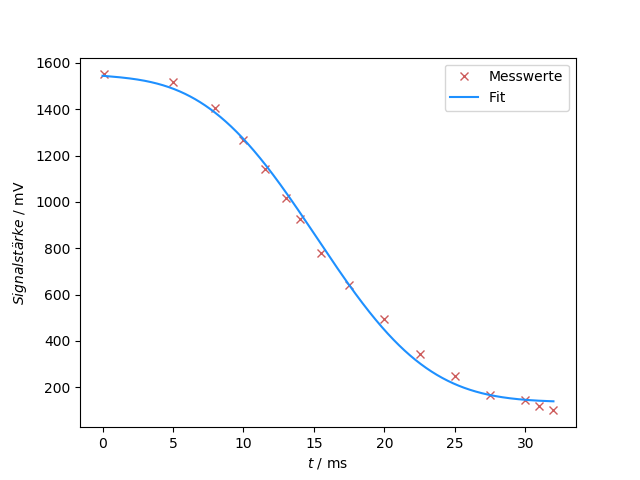
\includegraphics[width=0.8\textwidth]{../Auswertung/Diff_fit.png}
  \caption{Die gemessenen Echohöhen aufgetragen gegen den Pulsabstand $\tau$. Zur Bestimmung der Diffusionszeit $T_D$ wird eine
  Ausgleichskurve bestimmt.}
  \label{fig:diff_fit}
\end{figure} \noindent
Die Regression liefert
\begin{align}
  M_0 &= \SI{1.39(002)}{\volt} \\
  M_1 &= \SI{0.14(002)}{\volt} \\
  T_D &= \SI{5.33(025)e-6}{\second}
\end{align}
für die gesuchten Parameter.
Mithilfe des Zusammenhangs
\begin{equation}
  T_D = \frac{3}{2D\gamma^2 G^2}
\label{eqn:D}
\end{equation}
kann die Diffusionskonstante bestimmt werden. Dabei beschreibt G den Gradienten, der mittels Fouriertransformation eines Echos
bestimmt wird. In Abbildung \ref{fig:echo} ist das verwendete Echo dargestellt. Wobei sowohl der Imaginär- als auch der Realteil
zu sehen sind. Dieses Echo ist bereits phasenkorrigiert, daran zu erkennen, dass der Imaginärteil zu Beginn nicht verhanden ist.
\begin{figure}[H]
  \centering
  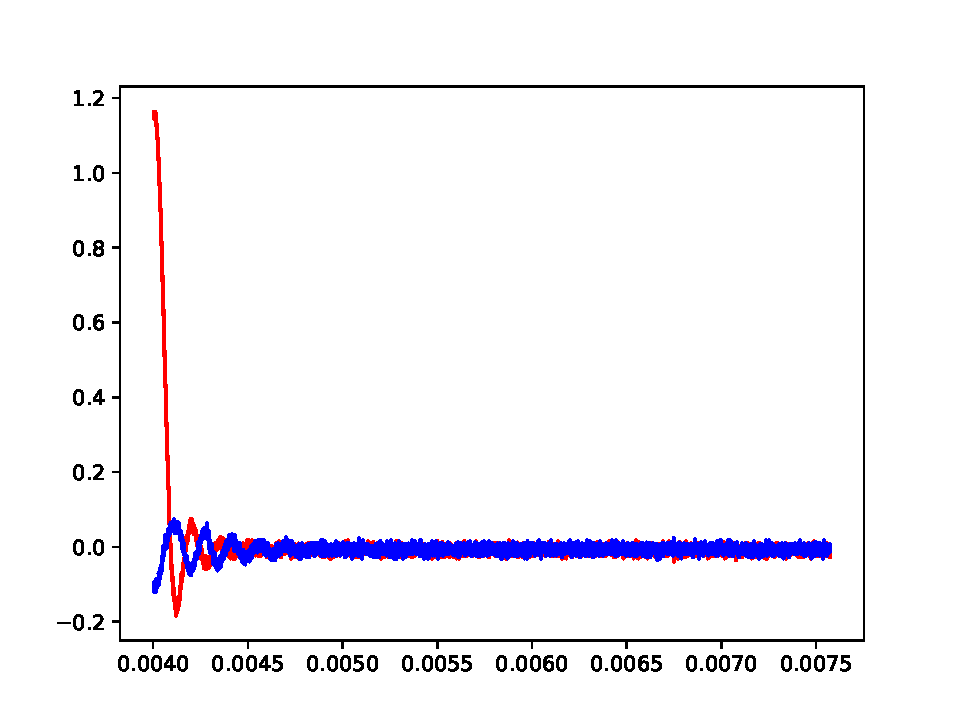
\includegraphics[width=0.9\textwidth]{../Auswertung/echo.pdf}
  \caption{Das zur Berechnung des Gradienten verwendete Echo nach einer Phasenkorrektur.}
  \label{fig:echo}
\end{figure} \noindent
In Abbildung \ref{fig:ft} ist das zu Abbildung \ref{fig:echo} gehörige Frequenzspektrum abgebildet, das mithilde der 
Fouriertransformation bestimmt wird. Dieses Spektrum gibt die Verteilung der Larmorfrequenzen innerhalb der Protonen wieder.
Aufgrund des geschalteten Gradienten unterscheidet diese sich abhängig vom Ort der Protons.
\begin{figure}[H]
  \centering
  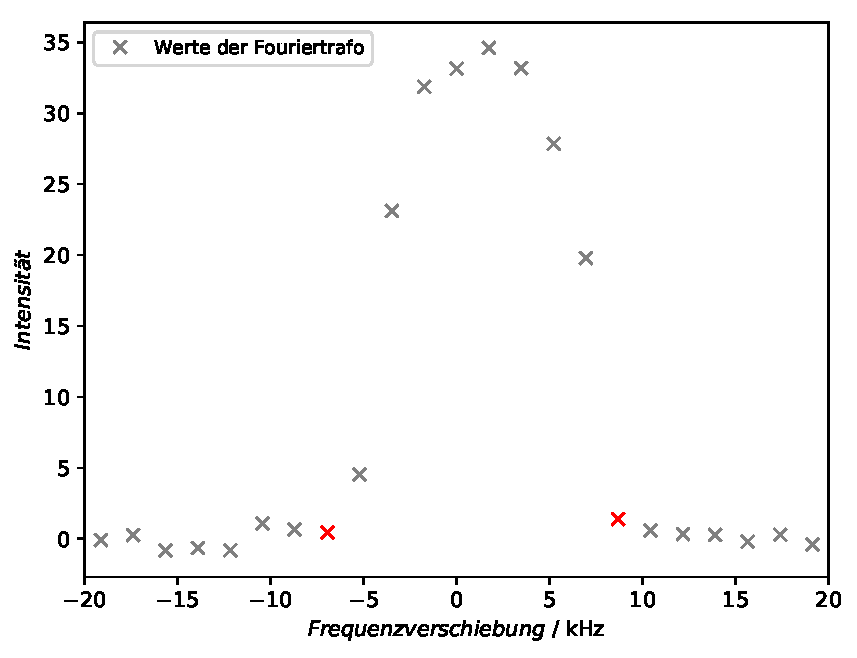
\includegraphics[width=0.9\textwidth]{../Auswertung/echo_ft.pdf}
  \caption{Das Ergebnis der auf das Echo angewendete Fouriertransformation. Mithilfe der Bestimmung der Breite der Frequenzverbreiterung
  ist es möglich den Gradienten und darüber die Diffusionskonstante zu berechnen.}
  \label{fig:ft}
\end{figure} \noindent
Mithilfe der Frequenzbreite, die in Abbildung \ref{fig:ft} zu 
\begin{align}
  d_f = \SI{1}{\kilo\hertz}
\end{align}
bestimmt wird, ist es über den Zusammenhang
\begin{align}
  G = \frac{s\pi d_f}{\gamma d}
\end{align}
möglich den vorliegenden Gradienten zu
\begin{align}
  G = \SI{1}{\tesla\per\meter}
\end{align}
zu bestimmen. Dabei wird mit $d = \SI{4.2}{\milli\meter}$ der Durchmesser des Probenröhrchens verwendet.
Mit dem bestimmten Grradienten und Gleichung \ref{eqn:D} kann die Diffusionskonstante zu 
\begin{align}
  D = \SI{1(01)}{\square\meter\per\second}
\end{align}
bestimmt werden.